\documentclass[11pt]{article}
\usepackage{amssymb}
\usepackage{algpseudocode}
\usepackage{algorithm}
\usepackage{setspace}
\usepackage{graphicx}
\graphicspath{ {./images/} }
\usepackage{hyperref}
\usepackage{siunitx}
\usepackage{amsmath}
\usepackage{caption}
\usepackage{subcaption}

\hypersetup{
    colorlinks=true,
    linkcolor=blue,
    filecolor=magenta,      
    urlcolor=cyan,
}

\title{MSc Project - Binding Affinity Prediction of Protein-Ligand Complex}
\author{
        Abdus Salam Khazi\\
        \href{mailto:abdus.khazi@students.uni-freiburg.de}
                {abdus.khazi@students.uni-freiburg.de}\\ \\
        \href{https://github.com/abduskhazi/MSc-Project}
                {Github Repository} \cite{github_repository} \\ \\
        Supervisors:
        \begin{tabular}{ll}
			Simon Bray \&
			Alireza Khanteymoori
		\end{tabular}
       }
	
\begin{document}

\maketitle
\date{}
\tableofcontents
\newpage

\section{Introduction}

\subsection{Biological Background}
Proteins are the workhorses of our body.  They are necessary for many important functions in the body.  Ligands are molecules that bind to proteins to form protein-ligand complexes.  They can be molecules that the protein transports (e.g., a Haemoglobin transporter) or act as stimulating agents.  In addition to this, they can also start/stop the protein from doing its function.  The correct functioning of these protein-ligand complexes is essential for any living organism.

The study of protein-ligand complexes is an intrinsic part of the drug discovery field.  It is because drugs are small molecules that act as ligands.  As the drug molecules (ligands) bind to the target proteins, they can artificially influence the protein behavior.  This causes a therapeutic effect.

\begin{figure}[htb]
  \centering
    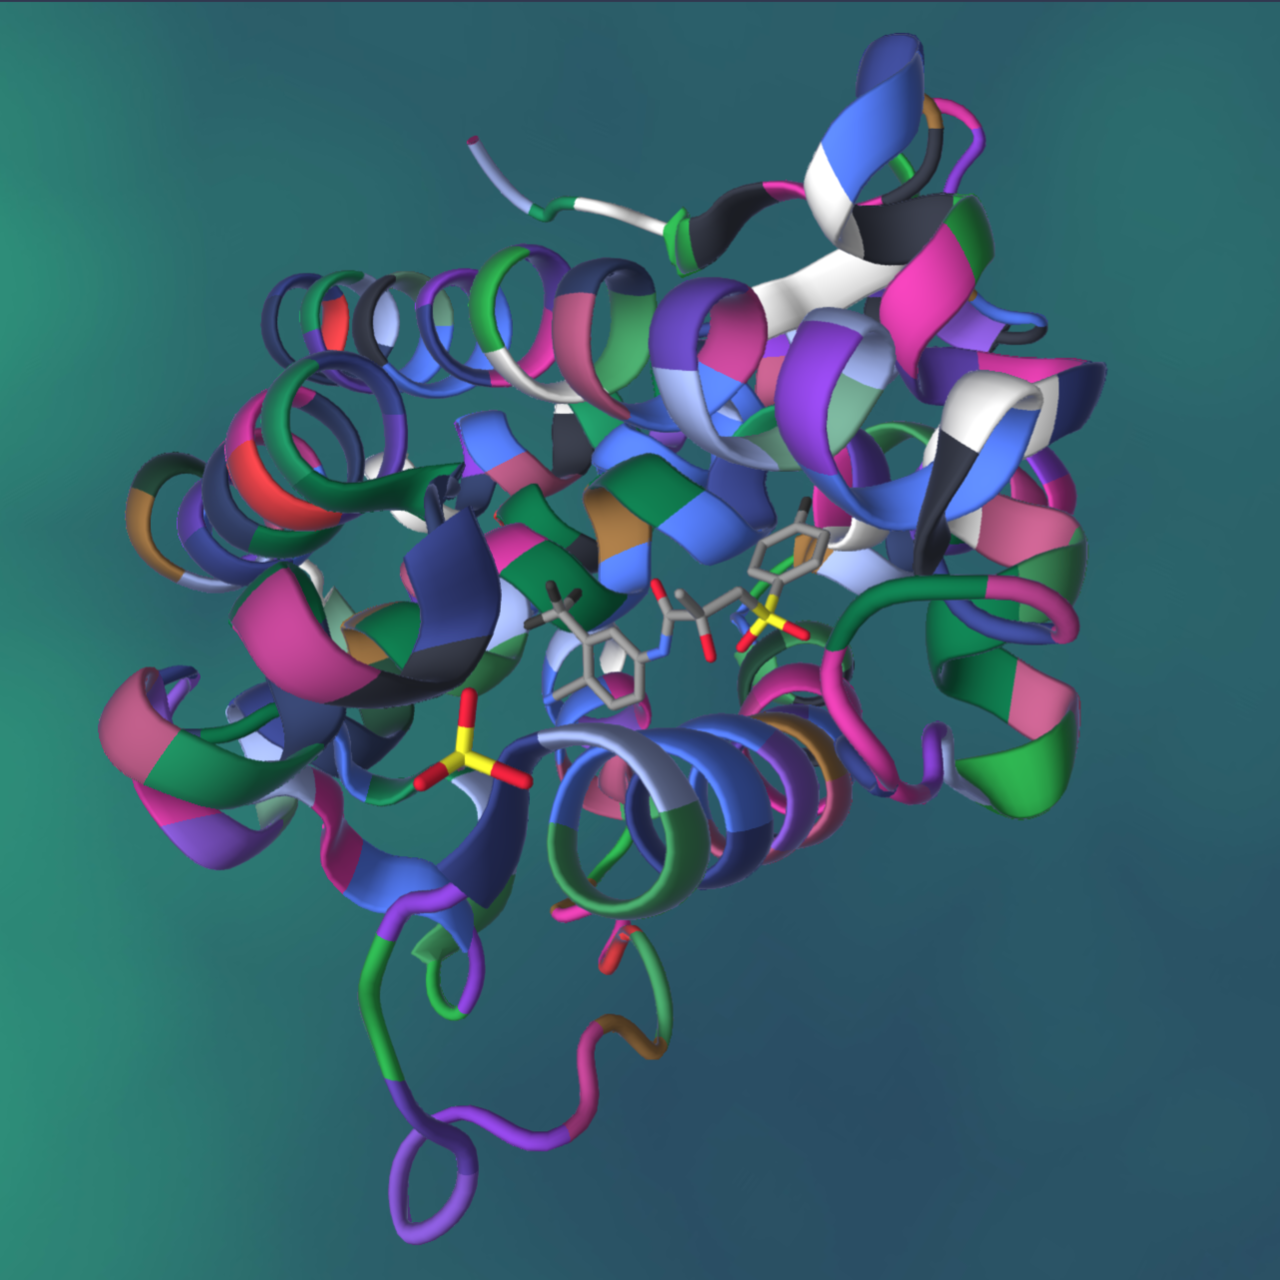
\includegraphics[scale=0.15]{images/pl_complex}
    \caption{Haemoglobin transporter protein.  \cite{PL_complex_introduction}}
    \label{fig:HaemoglobinTransporterImage}
\end{figure}


When we find a target drug candidate, we have to answer questions like - How easily does the drug bind to the target protein? Does it bind to any other protein - If so, is it desirable? Does it have any unforeseen effect on the protein function? etc...  To answer these questions biologists and pharmacists conduct wet-lab experiments that are expensive.

One way to reduce the cost of these experiments is to make a data-driven selection of the drugs.  Using experimental data collected over many years, one can build models to predict the behavior of the proposed drug computationally.  These 'In-Silico' computational methods can aid in the elimination of undesirable drugs as well as guide the drug selection process.

Our project aims to answer one of the above questions - How well does a given drug bind to the target protein? We determine this computationally by building a machine learning model that trains on the previous data.  We hope that this model will help reduce the costs of drug discovery. 

\subsection{Understanding Binding Affinity}
The binding affinity between a protein and a ligand is quantified by the $K_d$, $K_i$ and $IC_{50}$ measures in the PDBBind Data bank.
Here $K_d$ refers to disassociation constant, $K_i$ refers to the inhibition constant, and $IC_{50}$ refers to 
inhibitory concentration 50\%.
The reason for having different measurements is because it is not possible to use the same measurement techniques
for all biological complexes/processes.

To understand $K_d$, consider a protein and a ligand binding and unbinding continuously in a kinetic system.
In this system, let $[P]$, $[L]$, and $[PL]$ represent the concentrations of the Protein, the Ligand, and the Protein-Ligand complex respectively.
This is represented by the following equation:
$$[P] + [L] \rightleftharpoons [PL]$$
We can quantify the binding affinity $K_d$ by using the concentrations in the above system at equilibrium.
$$K_d = \frac{[P][L]}{[PL]} = \frac{k_{-1}}{k_1}$$
where $k_{-1}$ is the disassociation rate constant and $k_1$ is the association rate constant.
Similarly, $K_i$ and $IC_{50}$ are defined using concentration albeit non-trivially. 
\cite{binding_affinity_description}

\subsection{PDBBind Dataset}
Over the last few decades, researchers have been successful in building a single data archive for proteins.  This archive, called \textbf{Protein Data bank} \cite{pdb_homepage} , holds 3-D structural data of the proteins determined by experiments like X-ray crystallographic, Nuclear magnetic resonance (NMR), and cryoelectron microscopy (cryoEM).  A subset of this data also contains information about how well a given protein and ligand bind together.  It is called binding affinity between a protein and ligands.  (It also contains data about protein-protein complexes that our project does not deal with)
\cite{pdbank_history}

As we study the protein-ligand binding affinity here, we would like to filter out this data from the protein data bank.  It is what is done by the maintainers of the \textbf{PDBBind Data bank}.
\cite{pdbbind_introduction}
Using the curated protein-ligand affinity data present in the PDBBind Data bank, we build a machine learning model that learns to predict the affinity. 

\section{Problem Formulation}
\subsection{Problem Overview}
\label{ProblemOverviewlabel}
The problem that we are solving is - \textit{Given $K_d$/$K_i$/$IC_{50}$ for various complexes in the PDBBind Data bank,
can we predict this affinity measure for new protein-ligand complexes?}
Figure~\ref{fig:plproblemclassification} shows how the Protein-Ligand problem can be classified.

\begin{figure}[htb]
  \centering
    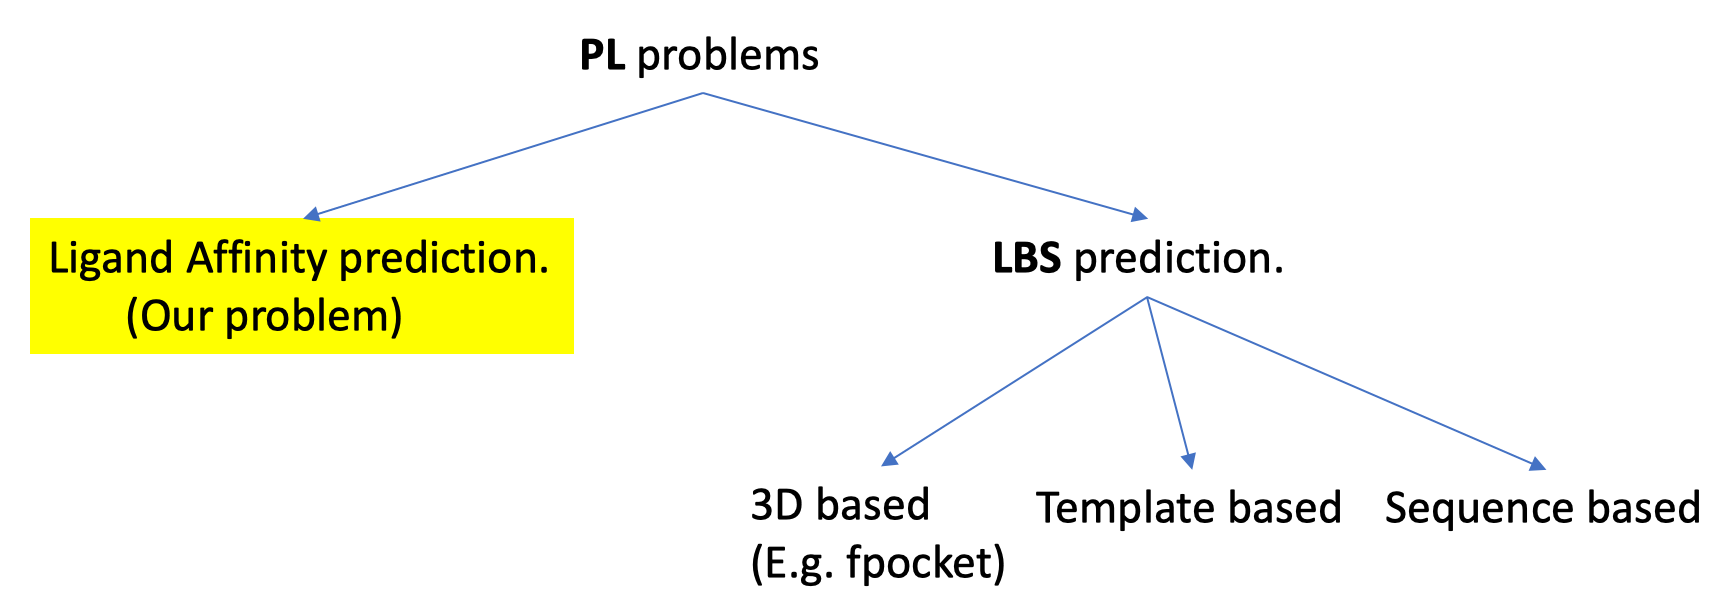
\includegraphics[scale=0.35]{images/pl_problem_classification}
    \caption{Protein-Ligand problem classifcation.}
    \label{fig:plproblemclassification}
\end{figure}

The binding of proteins and ligands is heavily influenced by their respective 3D structures.
Figure~\ref{fig:lockandkey} illustrates a hypothesis called \textit{Lock and Key}.
As you can see it is very crucial that the shape of the protein's binding location and the shape of the ligand be complementary for the binding.

\begin{figure}[htb]
  \centering
    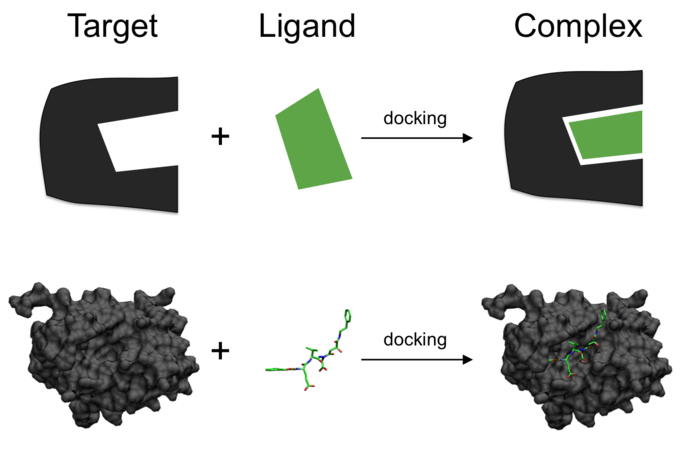
\includegraphics[scale=0.7]{images/lock_and_key}
    \caption{Lock and Key hypothesis in molecular docking.  \cite{lockandkeyformatpng}}
    \label{fig:lockandkey}
\end{figure}

The other parts of the protein are not involved in the binding process directly.
Hence,  we only get the features of the binding location.
Any potential binding location in the 3D structure of a protein is called a pocket.
We use a 3D based LBS prediction package called \textit{fpocket} to find the potential pockets.
A submodule in the package called \textit{dpocket} is used to extract the binding pocket's features.

To give a plug-and-play input to our model, we keep the features of proteins and ligands distinct till the training phase.
That is,  we do not use the combined features in any pre-processing of the ML pipeline e.g.  feature reduction.
This helps our model to provide the binding affinity between any protein and any ligand.



\subsection{Overview of file formats}
The \textbf{PDBBind Data bank} extracts information about the PL complexes from the \textbf{Protein Data bank} and creates the following files for every complex
\begin{itemize}
\item \textbf{PDB Format} - For the Protein.
\item  \textbf{Mol2} - For the ligand.
\item \textbf{SDF} - For the ligand.
\end{itemize}

All of the above formats contain the 3D information that is essential in the prediction of the binding affinity.
All the above mentioned formats use the \textbf{XYZ format} internally to represent the 3D structure of their molecules.

\subsubsection{XYZ format}
\label{xyz_format}
XYZ format is a chemical file format that represents the geometry of a molecule.
It specifies the number of atoms and their Cartesian X, Y, Z coordinates hence the name XYZ format.
The coordinates are relative to each other. Hence, translation and rotation do not change the molecule's representation. 
The following text illustrates the XYZ format.
Section \ref{XYZFileexampleref} gives an example.
\cite{XYZ_format}
\begin{verbatim}
<number of atoms>
comment line
<element> <X> <Y> <Z>
...
\end{verbatim}

The unit of distance used is Angstrom (\si{\angstrom}).  \SI{1}{\angstrom} $ = 10^{-10}$ m.
\cite{XYZ_format}

\subsubsection{PDB format}
PDB format is a human-readable file format used to represent the protein molecules (macromolecules).
Within the PDB format,  the coordinates of atoms are represented like the XYZ format [see \ref{xyz_format}].
Because of the 3D information in this format,  molecular visualization of proteins is possible with specialized software. 
It also contains information about atomic connectivity and the protein's primary,  secondary,  tertiary,  and quaternary structures.
\cite{pdb_file_format}
\cite{understanding_pdb_format}
Please see \cite{examplePDBFile} for an example pdb file.


\subsubsection{Structure Data File (SDF) Format}
SDF format file is a Chemical Table file (CT File) that contains structure of the molecule in the X,Y,Z format.
It contains information like atomic bonds,  connectivity information,  molecular weight,  and molecular formula. \cite{SDFformat}
Section \ref{SDFFileexampleref} illustrates the SDF file format.

\subsubsection{Mol2 format}
Similar to SDF format,  Mol2 also represents the 3D structure of a molecule in the X,Y,Z format.
It contains the atomic bond and connectivity information but does not contain the other data like molecular weight and formula.
We use the ligands given in this format because more ligands in mol2 format could be processed with the RDKit feature extractor.
Section \ref{MOL2Fileexampleref} illustrates the Mol2 file format.

\subsubsection{SMILES format}
SMILES is an acronym for Simplified Molecular-Input Line-Entry System.
It represents a molecule using an ASCII string.
Using the 3D data in SDF and Mol2 formats,  we can create an atomic graph representation.
Using this graph the SMILES string for the molecule can be generated.
The smiles format itself is not very helpful for us as we lose the 3D structural information after converting to it.
\cite{smilesformat}

\subsection{Extraction of features}
As the file formats are different for proteins and ligands,  we use different tools to extract their features.
\subsubsection{Ligand Features using RDKit}
RDKit is an open-source cheminformatics software \cite{rdkitofficalpage}.
The core data structures and algorithms of RDKit are written in C++ and the
python wrappers are generated using Boost.Python.
Using the module, \textit{RDKit.Chem.Descriptors} we extract $402$ features for each ligand \cite{rdkitbioinformaticsfreiburg}.
Each descriptor value is taken as a real number,  hence the input space of ligand features is $\mathbf{R}^{402}$ before any feature elimination.

\subsubsection{Protein Features using fpocket/dpocket descriptors}
\textit{Fpocket} stands for "Find pocket" whereas \textit{Dpocket} stands for "Describe pocket".
\textit{Fpocket} uses 3D Voronoi tessalation and the concepts of "Alpha Spheres" to find out pockets in the protein structure \cite{fpocketmanual} \cite{voronoitesselationshortvideo}.
Given a protein PDB file, we can extract the descriptors of all pockets in the protein.
For every pocket, we get 55 descriptors in total which are take as $\mathbf{R}$ values.
Hence the input space for protein features is $\mathbf{R}^{55}$.


To get the descriptors of the ligand-binding pockets,  we use \textit{Dpocket}.
\textit{Dpocket} is provided with the protein PDB file and the ligand ID of the PL complex as input.
It generates 3 files as output files,  namely,  dpout\_fpocketp.txt, dpout\_fpocketnp.txt,  and  dpout\_explicitp.txt.
\begin{itemize}
\item \textbf{dpout\_fpocketp.txt}.
This file contains the descriptors (a.k.a features) of all pockets that are considered to be binding pockets based on a binding criterion.
Multiple pockets can bind with the same ligand.
Hence,  there may be features of more than 1 pocket in this file.
\item \textbf{dpout\_fpocketnp.txt}.  This file contains the descriptors of all pockets that are non-binding according to the criteria.
\item \textbf{dpout\_explicitp.txt}.  An explicit pocket is defined as a pocket consisting of all vertices/atoms situated at a specific distance from the ligand in the PL complex.
This distance is 4 \r{A} by default.
This file contains the descriptors of all explicit pockets in the PL complex. 
\end{itemize}

In our project, we do not use dpout\_fpocketnp.txt as they contain non-binding pockets.
In the other 2 files,  we prefer using pocket descriptors given by dpout\_fpocketp.txt as explicitly defined pockets are heavily biased towards the ligand.

\section{Feature selection}
\subsection{Requirement of feature selection}
Both the protein and the ligand are equally responsible for the affinity of the PL complex.
Hence we concatenate their descriptors to get a high dementional $\mathbf{R}^{457}$ input for our model.
There are a couple of issues with using all of the descriptors.
\begin{itemize}
\item The amount of data is not very large. 
For example,  we could only get $\approx$ 35000 data points after concatenating the ligand features with the \textit{fpocketp} pocket descriptors.
\item The number of ligand descriptors $>>$ protein descriptors.
This creates a data imbalance and may lead the model to select only ligand features for their prediction.
\end{itemize}
Hence we need some methods to reduce the input dimensions.

\subsection{Feature Selection Strategies}

%The data if it is complementary is better for solving the problem.
%The accuracy measure of the protein LBS prediction is the same as the dichotomous problems in math.

We try to select features of the protein and the ligand separately.
This helps us make our model plug-and-play as discussed in section \ref{ProblemOverviewlabel}.
The best combination,  i.e Global Optima,  cannot be obtained practically by brute force algorithms.
This is because we would have to try $\binom{402}{k_1} * \binom{55}{k_1}$ ($k_1, k_2 \in \mathbf{I}^+$) possibilities which is impractical.
The following feature selection heuristics were used instead -

\subsubsection{Selection by output correlation}
The \textit{pearson} and \textit{spearmann} correlations of each feature were calculated against the output variable.
We assumed that the features were either linearly related to the output (in the case of pearson correlation) or had a monotonic relationship (in the case of spearmann correlation).
The features with the highest correlation were selected as inputs to the model.

\subsubsection{Using genetic algorithms \cite{genetic_algorithm}}
Since the feature space is a non-continuous problem of combinatorial complexity,
we also studied genetic feature selection algorithms.
We represent each feature by a binary number, 1 for inclusion of feature and 0 for the exclusion.
Each feature selection $p \in \mathbb{B}^{456}$ (401 for ligands + 55 for proteins) is called a chromosome.
A "population" of $n$ chromosomes is maintained.
For each generation,  the best pairs of chromosomes are selected as parents.
The next generation is created by crossover and mutation of the chromosomes.
Algorithm~\ref{alg:GeneticAlgo} below gives a complete pseudocode for this.

The scoring function used to select the best chromosome can vary according to the type of the model being fit. [See Section~\ref{MachineLearningModelslabel}]

\subsubsection{Manual Feature selection}
Features selected by expert. Given by Simon Bray. (Yet to do)

\begin{algorithm}
\caption{Selection of features in our model using genetic algorithm \cite{genetic_algorithm}}
\label{alg:GeneticAlgo}
\begin{algorithmic}[1]
\Procedure{GENETIC\_ALGORITHM\_BASED\_SELECTOR}{}
\State scoringfunction $\gets$ Get model specific scoring function
\State $ population = \{C_1, C_2, C_3... C_n\}$ $\in$ $\mathbb{B}^{456}$ (initial chromosomes).
\State best $\gets C_1$  \textit{// Arbitrarily initialized}
\State $i \gets 0$
\State $gen \gets$ number of generations to run.
      \For{\texttt{$i < gen$ with step 1}}
          \State $\{S_1, S_2, S_3... S_n\} \gets$ scoringfunction($population$) $\forall S_i \in \mathbf{R}$.
          \State \textit{// Do a tournament selection for the best chromosomes}
          \State $genetically\_better\_population \gets$ empty list
          \For{\texttt{$j < len(population)$}}
              \State Set $\gets$ random\_k\_selections($population$)
              \State $c \gets best($Set$)$ \textit{// Based on scoringfunction.}
              \State $genetically\_better\_population.add(c)$
          \EndFor
          \State $children \gets$ empty list
          \For{\texttt{$j < len(population)$ with step 2}}
              \State $P_1, P_2$ $\gets$ $population[j], population[j+1]$
              \State $c_1, c_2 \gets crossover(P_1, P_2)$
              \State $c_1 \gets mutation(c_1)$
              \State $c_2 \gets mutation(c_2)$
              \State $children.add(c_1, c_2)$
          \EndFor
          \State $population \gets children$
      \EndFor
\State return best($population$)
\EndProcedure
\end{algorithmic}
\end{algorithm}

\section{Testing}
\subsection{Reproducibility}
Reproducible ML models are very crucial for verifying any project or research results. Due to the stochastic nature of many ML training processes, reproducing the exact model (and consequently the exact output) is a challenge. Two methods can be employed to produce verifiable results:
\begin{itemize}
\item Training many models and reporting the average results.
\item Controlling the randomness of the trained models. It is done by setting the seed of the pseudo-random algorithms.
\end{itemize}

We use the second approach in our project. Every script, when executed, reports an execution ID. This is the random seed used during the execution. If we want to reproduce the exact results, we give this execution ID to the script as the first argument.

\subsection{Model Quality Analysis}
We are trying to predict the following function
$$ \textrm{Binding affinity prediction} : \mathbf{R}^n \mapsto \mathbf{R} \;\; \textrm{where} \;\; n \in \mathbf{I}^+$$
Since the input space is multi-dimensional, we cannot fully visualize our model as a function of the input space.
To get around this using the following methods
\begin{itemize}
\item We report \textit{Coefficient of determination}, $R^2  \in (- \infty, 1.0]$ where $1.0$ is the best score. \cite{r_squared_score}
$$R^2(y, \hat{y}) = 1 - \frac{\sum_{i=1}^{n} (y_i - \hat{y}_i)^2}{\sum_{i=1}^{n} (y_i - \bar{y})^2} \;\; \textrm{where} \;\; \bar{y} = \frac{1}{n} \sum_{i=1}^{n} y_i \;\;
\textrm{and} \;\; \sum_{i=1}^{n} (y_i - \hat{y}_i)^2 = \sum_{i=1}^{n} \epsilon_i^2$$

\item For visualizing the results,  we plot a 2D plot of expected values against the model's output. 
\end{itemize}

A perfect model would have all the points on the $y = x$ line.  This corresponds to $R^2$ score of $1.0$. 
Figure~\ref{fig:modelQualityVisualization},  shows the validation accuracy of a sample \textit{Random Forest Regressor} model.
$y\_validate$ ($x$ axis) represents the actual validation data.
$y\_validate\_pred$ ($y$ axis) represents the predicted output from the model.

\begin{figure}[htb]
  \centering
    \includegraphics[width=1.0\textwidth]{images/accuracy_validate}
    \caption{(Sample) Visualizing accuracy.  $R^2 \approx 0.805$.}
    \label{fig:modelQualityVisualization}
\end{figure}

%\includegraphics[scale=0.7]{accuracy_validate}
%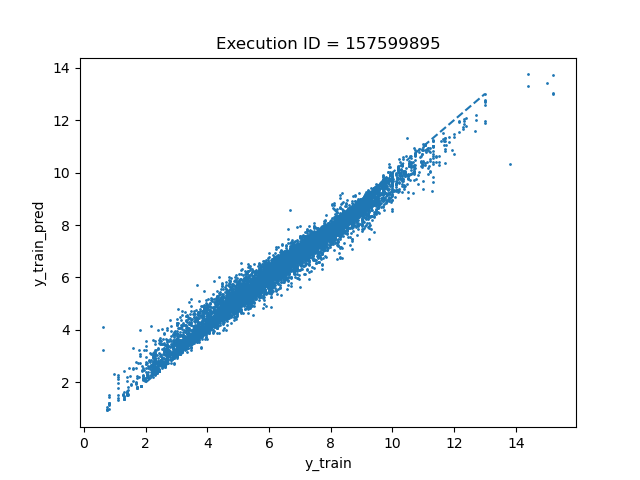
\includegraphics[scale=0.7]{accuracy_train}

\section{Machine Learning Models}
\label{MachineLearningModelslabel}
Various machine learning models were trained using the extracted data.
We tried out Linear Regression,
Support Vector Regression,
a small Neural Network,
as well as a Random Forest Regression.
But by far the most impressive performance was given by Random Forest Regression.

\subsection{Linear regression}
Linear regression fits a linear model to a given data.
It tries to minimize the square of errors between the predicted output value and the actual output value.
This is the cheapest model (computationally) that we used to fit our data.
Table~\ref{table:1} shows the overview of our analysis with this model.
Figure~\ref{fig:BestLinearModel} shows the best results obtained with linear regression.

\begin{table} [h!]
\centering
 \begin{tabular}{ | c | c | c | c | }
\hline
\textbf{Features Selected} & \textbf{Training $R^2$ Score} & \textbf{Validation $R^2$ Score} \\ [0.5 ex]
\hline \hline
457 (all) & 0.458 & 0.414\\
50 (Genetic - Random init)\footnotemark[1] & $\approx$0.379 & $\approx$0.359\\
49 (Genetic - Specific init)\footnotemark[1] & $\approx$0.378 & $\approx$0.368  \\
- (Output Correlation) & - & -  \\ 
- (manual) & - & -  \\ [1ex]
\hline
\end{tabular}
\caption{Simple linear model overview}
\label {table:1}
\end{table}

\begin{figure}
     \centering
     \begin{subfigure}[b]{0.45\textwidth}
         \centering
         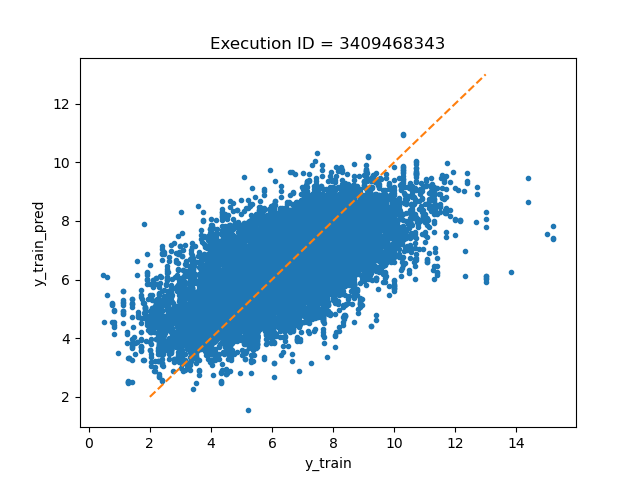
\includegraphics[scale=0.45]{images/accuracy_train_all_linear}
         \caption{Training Accuracy ($R^2 \approx 0.458$)}
        \label{fig:TrainingAccuracyLinearModel}
     \end{subfigure}
     \hfill
     \begin{subfigure}[b]{0.45\textwidth}
         \centering
         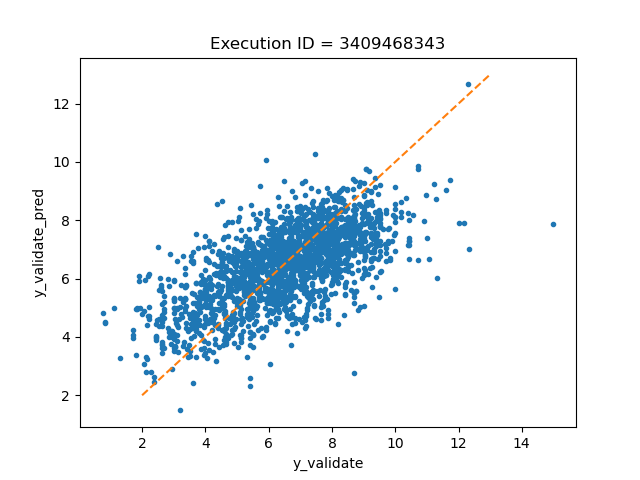
\includegraphics[scale=0.45]{images/accuracy_validate_all_linear}
        \caption{Validation Accuracy ($R^2 \approx 0.414$)}
        \label{fig:ValidationAccuracyLinearModel}
     \end{subfigure}
     \caption{Best Linear Model.  All 457 features selected.}
     \label{fig:BestLinearModel}
\end{figure}

The reason for the low $R^2$ score is that linear models assume a strong linearity between the input variables and the output variable.
This is not always true.

\subsubsection{Score function of genetic feature selection}
Since the fitting of the linear regression model was very cheap, we could afford to refit the model every time in our genetic algorithm.
We had 2 objectives at hand
\begin{itemize}
\item Get the best performing model.
\item Reduce the number of input features to make our model simple and explainable.
\end{itemize}
The above objectives may not completely be against each other.
This is because removing a feature that has no correlation (or random correlation) with the output may improve the model whereas removing a feature that the output is highly correlated on degrades the model.

\footnotetext[1]{Approximately reproducible as the reproducibility module was introduced later.}

Hence,  taking inspiration from the hypervolume-based multi-objective optimization, we designed the following score function.
$$
\textrm{score} = \mathbf{R}^2 * \textrm{Features Eliminated}
$$
Figure~\ref{fig:scorefunctionfigure} gives us an intuition about this function.
Here the score function represents the area of the square formed between a given point and the origin.
Trying to improve the score means,  it will try to eliminate more features as well as try to get a higher $R^2$ score.
In the example below,  the point $a$ is preferred over $b$ as it gives almost the same $R^2$ score and eliminates a larger number of features.
Another advantage of this score function is that the scale of both axes is irrelevant.

\begin{figure}[htb]
  \centering
    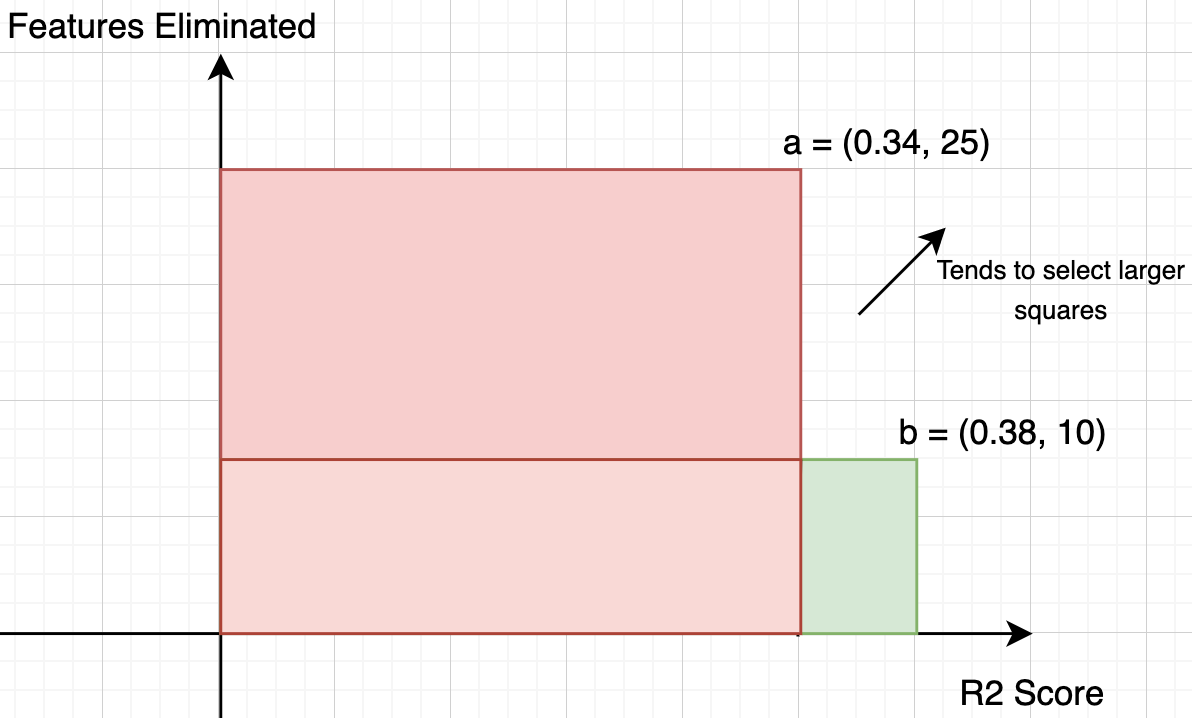
\includegraphics[scale=0.5]{images/scoreFuntionMultiObject}
    \caption{Genetic Algorithm score function representation.}
    \label{fig:scorefunctionfigure}
\end{figure}

\subsubsection{Initialization strategies of population}
Two main strategies were used to initialize the population for the genetic algorithm
\begin{itemize}
\item \textbf{Random Initialization}.  A population of $2400$ chromosomes was randomly initialized and run for $500$ generations.
\item \textbf{Specific Initialization}.  Here,  the initial population was kept at $457$.
The algorithm was run for $2000$ generations.
Each chromosome in the population had 1 distinct feature excluded.  The following represents the initialization of the chromosomes.

$
c_1 = [0 1 1 1 1 ......  1 1]
$ \\
$
c_2 = [1 0 1 1 1 ......  1 1]
$ \\
$
c_3 = [1 1 0 1 1 ......  1 1]
$ \\
$
... 
$ \\
$
c_{457} = [1 1 1 1 1 ......  1 0]
$

The rationale was that using the above score function we could go to a local minimum by eliminating the worst performing features rather than trying to select the best performing features as in the case of random initialization.
\end{itemize}

Both the initialization strategies gave similar results as shown in Table~\ref{table:1}

\subsection{Random Forest Regression}
A random forest regression is an ensemble model which uses an ensemble of trees
to calculate the output variable.
Each node in the tree reduces tries to reduce the entropy of the data at hand.
The $R^2$ score we got was $> 0.75$ for an ensemble of $100$ trees.

\subsubsection{Feature Importance calculation}
The Random Forest regression model fitting is very expensive as compared to the simple linear regression.
Hence the same strategy cannot be used for feature selection as used in the linear models.
We used 2 main methods to determine the importance of features in the model
\begin{itemize}
\item \textbf{Gini Importance} - This is given by default by the model. The model 
calculates the amount of entropy reduction of that each feature does when it divides the data using the OOB score. (Out of bag Score)
\item \textbf{Permutation Importance} - This is a model agnostic method to determine the importance of features in a regression. 
It tries to calculate the reduction in the accuracy we shuffle each column.
\end{itemize}
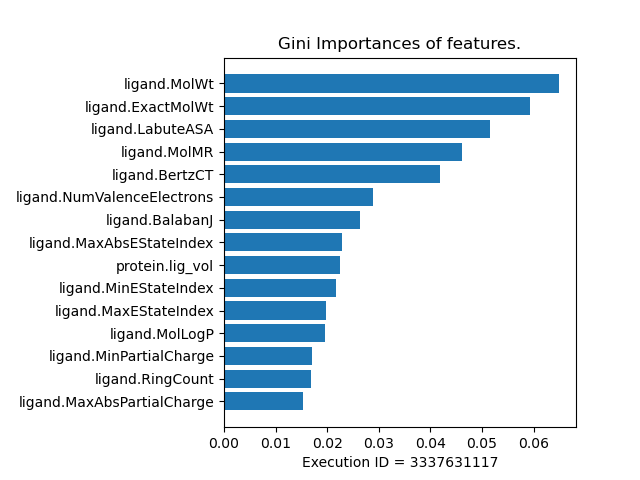
\includegraphics[scale=0.7]{Gini_importance}

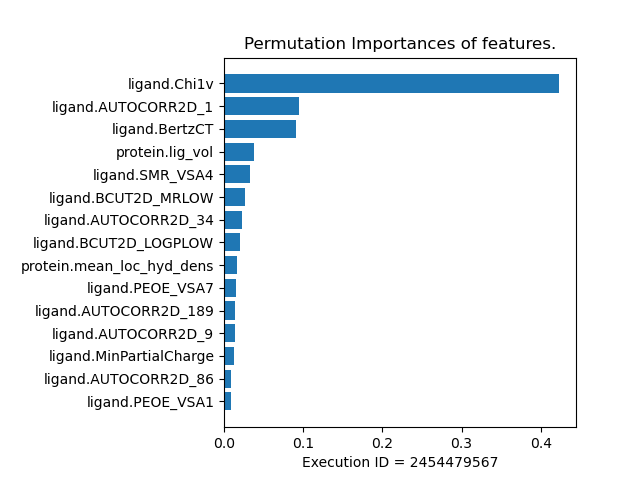
\includegraphics[scale=0.7]{Permutation_importance}

The issue with the above methods is that if there is any hidden correlation between input features then it will reduce the importance of the correlated features.

\subsection{Permutation Importance and genetic algorithm}
To overcome the issue with the above feature importance selection, we plan to use a combination of the concepts of permutation importance and genetic algorithm to find out the importance of the selected features.

Results - YET TO IMPLEMENT

\section{Discussion}


\section{Conclusion}

\bibliographystyle{plain}
\bibliography{references}

\section{Appendix}
\subsection{XYZ File format}
\label{XYZFileexampleref}
The following represents the pyridine molecule in the XYZ format.
\begin{verbatim}
11

C       -0.180226841      0.360945118     -1.120304970
C       -0.180226841      1.559292118     -0.407860970
C       -0.180226841      1.503191118      0.986935030
N       -0.180226841      0.360945118      1.29018350
C       -0.180226841     -0.781300882      0.986935030
C       -0.180226841     -0.837401882     -0.407860970
H       -0.180226841      0.360945118     -2.206546970
H       -0.180226841      2.517950118     -0.917077970
H       -0.180226841      2.421289118      1.572099030
H       -0.180226841     -1.699398882      1.572099030
H       -0.180226841     -1.796059882     -0.917077970
\end{verbatim}

\subsection{SDF File format}
\label{SDFFileexampleref}
\begin{verbatim}
2uzn_ligand

Created by X-TOOL on Fri Nov 18 14:55:27 2016
 37 39  0  0  0  0  0  0  0  0999 V2000
    7.1480   60.4530    6.6830  O 0  0  0  1  0  1
    6.0470   60.1670    7.5640  S 0  0  0  1  0  4
    .......
    .......
   -2.6338   67.4589    8.1225  H 0  0  0  1  0  1
  1  2  2  0  0  2
  2  3  2  0  0  2
  .......
  .......
 23 37  1  0  0  2
M  END
> <MOLECULAR_FORMULA>
C15H13N3O4S2

> <MOLECULAR_WEIGHT>
363.3

> <NUM_HB_ATOMS>
7  

> <NUM_ROTOR>
1  

> <XLOGP2>
1.31 
\end{verbatim}

\subsection{MOL2 File Format}
\label{MOL2Fileexampleref}
\begin{verbatim}
### 
### Created by X-TOOL on Fri Sep 26 17:34:18 2014
### 

@<TRIPOS>MOLECULE
1fo2_ligand
   25    25     1     0     0
SMALL
GAST_HUCK


@<TRIPOS>ATOM
      1 C4         39.0090   40.2680   25.5130 C.3       1 DMJ         0.1280
      2 O4         39.2170   40.5810   26.8980 O.3       1 DMJ        -0.3835
     .......
     25 H14        38.0787   41.8134   21.3802 H         1 DMJ         0.2097
@<TRIPOS>BOND
     1    1    9 1  
     2    1    3 1  
    .......
    25   11   25 1  
@<TRIPOS>SUBSTRUCTURE
     1 DMJ         1
\end{verbatim}

\end{document}
